% !TeX root = ../main.tex
\documentclass[class=article]{standalone}

\begin{document}
\section*{Question 1}

\subsection*{(a)}

\begin{center}
  \begin{tabular}{|rcl|rcl|}
      \hline
      \multicolumn{3}{|c}{\bf Productions} &
      \multicolumn{3}{|c|}{\bf Règles Sémantiques} \\
      \hline
      \hline
      $S$ & $\rightarrow$ & $A$ & $S.ok$ & $:=$ & $(A.sb \geq 1) \wedge (A.sc \geq 2)  $\\
      \hline
      $A$ & $\rightarrow$ & \lstinline[]$a$ $A_1$ & $A.sb$ & $:=$ & $A_1.sb$\\
          &               &                       & $A.sc$ & $:=$ & $A_1.sc$\\
      \hline
      $A$ & $\rightarrow$ & \lstinline[]$b$ $A_1$ & $A.sb$ & $:=$ & $A_1.sb + 1$\\
          &               &                       & $A.sc$ & $:=$ & $A_1.sc$\\
      \hline
      $A$ & $\rightarrow$ & \lstinline[]$c$ $A_1$ & $A.sb$ & $:=$ & $A_1.sb$\\
          &               &                       & $A.sc$ & $:=$ & $A_1.sc + 1$\\
      \hline
      $A$ & $\rightarrow$ & $\epsilon$ & $A.sb$ & $:=$ & $0$\\
          &               &            & $A.sc$ & $:=$ & $0$\\
      \hline
  \end{tabular}
\end{center}

\pagebreak

Vérification positive avec le mot $bcc \in L_1$

\begin{center}
  \begin{tikzpicture}
    [
    sibling distance=2em, level distance=40pt]

    \tikzset{edge from parent/.style={draw, edge from parent path=
    {(\tikzparentnode) -- (\tikzchildnode)}}}
    \Tree 
    [.$S\tbox{ok}{true}$ 
      [.$A\tbox{sb}{1}\tbox{sc}{2}$
        [.$A_1\tbox{sb}{1}\tbox{sc}{2}$
          b
          [.$A_2\tbox{sb}{0}\tbox{sc}{2}$
            c
            [.$A_3\tbox{sb}{0}\tbox{sc}{1}$
              c
              [.$A_4\tbox{sb}{0}\tbox{sc}{0}$
                $\epsilon$
              ]
            ]
          ]
        ]
      ]
    ]
  \end{tikzpicture}
\end{center}

Vérification négative avec le mot $\epsilon \notin L_1$
\begin{center}
  \begin{tikzpicture}
    [
    sibling distance=2em, level distance=40pt]

    \tikzset{edge from parent/.style={draw, edge from parent path=
    {(\tikzparentnode) -- (\tikzchildnode)}}}
    \Tree 
    [.$S\tbox{ok}{false}$ 
      [.$A\tbox{sb}{0}\tbox{sc}{0}$
        $\epsilon$
      ]
    ]
  \end{tikzpicture}
\end{center}

\pagebreak

\subsection*{(b)}
\begin{center}
  \begin{tabular}{|rcl|rcl|}
      \hline
      \multicolumn{3}{|c}{\bf Productions} &
      \multicolumn{3}{|c|}{\bf Règles Sémantiques} \\
      \hline
      \hline
      $S$ & $\rightarrow$ & $A$ & $A.hprev$ & $:=$ & \lstinline[]$""$\\
          &               &     & $S.ok$    & $:=$ & $A.ok $\\
      \hline
      $A$ & $\rightarrow$ & \lstinline[]$a$ $A_1$ & $A_1.hprev$ & $:=$ & \lstinline[]$"a"$\\
          &               &                       & $A.ok$      & $:=$ & $A_1.ok \wedge A.hprev \neq $\lstinline[]$"a"$\\
      \hline
      $A$ & $\rightarrow$ & \lstinline[]$b$ $A_1$ & $A_1.hprev$ & $:=$ & \lstinline[]$"b"$\\
          &               &                       & $A.ok$      & $:=$ & $A_1.ok\wedge A.hprev \neq $\lstinline[]$"b"$\\
      \hline
      $A$ & $\rightarrow$ & \lstinline[]$c$ $A_1$ & $A_1.hprev$ & $:=$ & \lstinline[]$"c"$\\
          &               &                       & $A.ok$      & $:=$ & $A_1.ok\wedge A.hprev \neq $\lstinline[]$"c"$\\
      \hline
      $A$ & $\rightarrow$ & $\epsilon$ & $A.ok$ & $:=$ & \lstinline[]$true$\\
      \hline
  \end{tabular}
\end{center}

Vérification positive avec le mot $\epsilon \in L_2$

\begin{center}
  \begin{tikzpicture}
    [
    sibling distance=2em, level distance=40pt]

    \tikzset{edge from parent/.style={draw, edge from parent path=
    {(\tikzparentnode) -- (\tikzchildnode)}}}
    \Tree 
    [.$S\tbox{ok}{true}$ 
      [.$\tbox{hprev}{""}A\tbox{ok}{true}$
        $\epsilon$
      ]
    ]
  \end{tikzpicture}
\end{center}

Vérification positive avec le mot $aa \notin L_2$

\begin{center}
  \begin{tikzpicture}
    [
    sibling distance=2em, level distance=40pt]

    \tikzset{edge from parent/.style={draw, edge from parent path=
    {(\tikzparentnode) -- (\tikzchildnode)}}}
    \Tree 
    [.$S\tbox{ok}{false}$ 
      [.$\tbox{hprev}{""}A\tbox{ok}{false}$
        a
        [.$\tbox{hprev}{"a"}A\tbox{ok}{false}$
          a
          [.$\tbox{hprev}{"a"}A\tbox{ok}{true}$
            $\epsilon$
          ]
        ]
      ]
    ]
  \end{tikzpicture}
\end{center}

\pagebreak

\subsection*{(c)}

\begin{center}
  \begin{tabular}{|rcl|rcl|}
      \hline
      \multicolumn{3}{|c}{\bf Productions} &
      \multicolumn{3}{|c|}{\bf Règles Sémantiques} \\
      \hline
      \hline
      $S$ & $\rightarrow$ & $A$ & $S.ok$ & $:=$ & $(247 + 12 * A.si = 23 * A.si + 7 * A.sk)$\\
      \hline
      $A$ & $\rightarrow$ & \lstinline[]$a$ $A_1$ & $A.si$ & $:=$ & $A_1.si + 1$\\
          &               &                       & $A.sj$ & $:=$ & $A_1.sj$\\
          &               &                       & $A.sk$ & $:=$ & $A_1.sk$\\
      \hline      
      $A$ & $\rightarrow$ & $B$ & $A.si$ & $:=$ & $0$\\
          &               &     & $A.sj$ & $:=$ & $B.sj$\\
          &               &     & $A.sk$ & $:=$ & $B.sk$\\
      \hline
      $B$ & $\rightarrow$ & \lstinline[]$b$ $B_1$ & $B.sj$ & $:=$ & $B_1.sj + 1$\\
          &               &                       & $B.sk$ & $:=$ & $B_1.sk$\\
      \hline
      $B$ & $\rightarrow$ & $C$ & $B.sj$ & $:=$ & $0$\\
          &               &     & $B.sk$ & $:=$ & $C.sk$\\
      \hline
      $C$ & $\rightarrow$ & \lstinline[]$c$ $C_1$ & $C.sk$ & $:=$ & $C_1.sk + 1$\\
      \hline
      $C$ & $\rightarrow$ & $\epsilon$& $C.sk$ & $:=$ & $0$\\
      \hline
  \end{tabular}
\end{center}


Vérification positive avec le mot $\epsilon \notin L_3$
\begin{center}
  \begin{tikzpicture}
    [
    sibling distance=1em, level distance=25pt]

    \tikzset{edge from parent/.style={,draw, edge from parent path=
    {(\tikzparentnode) -- (\tikzchildnode)}}}
    \Tree 
    [.$S\tbox{ok}{true}$ 
      [.$A\tbox{si}{0}\tbox{sj}{0}\tbox{sk}{0}$
        [.$B\tbox{sj}{0}\tbox{sk}{0}$
          [.$C\tbox{sk}{0}$
            $\epsilon$
          ]
        ]
      ]
    ]
  \end{tikzpicture}
\end{center}

Vérification positive avec le mot $aaabbbbbbbbbbbbc \in L_3$

{\hfill [Voir page suivante] \hfill}

{\hspace{-3cm}
  \begin{tikzpicture}
    [
    sibling distance=1em, level distance=25pt]

    \tikzset{edge from parent/.style={,draw, edge from parent path=
    {(\tikzparentnode) -- (\tikzchildnode)}}}
    \Tree 
    [.$S\tbox{ok}{true}$ 
      [.$A\tbox{si}{3}\tbox{sj}{12}\tbox{sk}{1}$
        a
        [.$A_1\tbox{si}{2}\tbox{sj}{12}\tbox{sk}{1}$
        a
        [.$A_2\tbox{si}{1}\tbox{sj}{12}\tbox{sk}{1}$
        a
        [.$A_3\tbox{si}{0}\tbox{sj}{12}\tbox{sk}{1}$
          [.$B\tbox{sj}{12}\tbox{sk}{1}$
            b
            [.$B_1\tbox{sj}{11}\tbox{sk}{1}$
            b
            [.$B_2\tbox{sj}{10}\tbox{sk}{1}$
            b
            [.$B_3\tbox{sj}{9}\tbox{sk}{1}$
            b
            [.$B_4\tbox{sj}{8}\tbox{sk}{1}$
            b
            [.$B_5\tbox{sj}{7}\tbox{sk}{1}$
            b
            [.$B_6\tbox{sj}{6}\tbox{sk}{1}$
            b
            [.$B_7\tbox{sj}{5}\tbox{sk}{1}$
            b
            [.$B_8\tbox{sj}{4}\tbox{sk}{1}$
            b
            [.$B_9\tbox{sj}{3}\tbox{sk}{1}$
            b
            [.$B_10\tbox{sj}{2}\tbox{sk}{1}$
            b
            [.$B_11\tbox{sj}{1}\tbox{sk}{1}$
            b
            [.$B_12\tbox{sj}{0}\tbox{sk}{1}$
              [.$C\tbox{sk}{1}$
                c
                [.$C_1\tbox{sk}{0}$
                  $\epsilon$
                ]
              ]
            ]
            ]
            ]
            ]
            ]
            ]
            ]
            ]
            ]
            ]
            ]
            ]
          ]
          ]
          ]
        ]
      ]
    ]
  \end{tikzpicture}
}

\end{document}